%% 
%% Copyright 2007-2024 Elsevier Ltd
%% 
%% This file is part of the 'Elsarticle Bundle'.
%% ---------------------------------------------
%% 
%% It may be distributed under the conditions of the LaTeX Project Public
%% License, either version 1.3 of this license or (at your option) any
%% later version.  The latest version of this license is in
%%    http://www.latex-project.org/lppl.txt
%% and version 1.3 or later is part of all distributions of LaTeX
%% version 1999/12/01 or later.
%% 
%% The list of all files belonging to the 'Elsarticle Bundle' is
%% given in the file `manifest.txt'.
%% 
%% Template article for Elsevier's document class `elsarticle'
%% with numbered style bibliographic references
%% SP 2008/03/01
%% $Id: elsarticle-template-num.tex 249 2024-04-06 10:51:24Z rishi $
%%
\documentclass[final,5p,times,twocolumn]{elsarticle}

%% Use the option review to obtain double line spacing
%% \documentclass[authoryear,preprint,review,12pt]{elsarticle}

%% Use the options 1p,twocolumn; 3p; 3p,twocolumn; 5p; or 5p,twocolumn
%% for a journal layout:
%% \documentclass[final,1p,times]{elsarticle}
%% \documentclass[final,1p,times,twocolumn]{elsarticle}
%% \documentclass[final,3p,times]{elsarticle}
%% \documentclass[final,3p,times,twocolumn]{elsarticle}
%% \documentclass[final,5p,times]{elsarticle}
%% \documentclass[final,5p,times,twocolumn]{elsarticle}

%% For including figures, graphicx.sty has been loaded in
%% elsarticle.cls. If you prefer to use the old commands
%% please give \usepackage{epsfig}

%% The amssymb package provides various useful mathematical symbols
\usepackage{amssymb}
%% The amsmath package provides various useful equation environments.
\usepackage{amsmath}
%% The amsthm package provides extended theorem environments
%% \usepackage{amsthm}

%% The lineno packages adds line numbers. Start line numbering with
%% \begin{linenumbers}, end it with \end{linenumbers}. Or switch it on
%% for the whole article with \linenumbers.
%% \usepackage{lineno}

\journal{Nuclear Physics B}

\begin{document}

\begin{frontmatter}

%% Title, authors and addresses

%% use the tnoteref command within \title for footnotes;
%% use the tnotetext command for theassociated footnote;
%% use the fnref command within \author or \affiliation for footnotes;
%% use the fntext command for theassociated footnote;
%% use the corref command within \author for corresponding author footnotes;
%% use the cortext command for theassociated footnote;
%% use the ead command for the email address,
%% and the form \ead[url] for the home page:
%% \title{Title\tnoteref{label1}}
%% \tnotetext[label1]{}
%% \author{Name\corref{cor1}\fnref{label2}}
%% \ead{email address}
%% \ead[url]{home page}
%% \fntext[label2]{}
%% \cortext[cor1]{}
%% \affiliation{organization={},
%%             addressline={},
%%             city={},
%%             postcode={},
%%             state={},
%%             country={}}
%% \fntext[label3]{}

\title{Digital twin}
% Digital Twin Modelling of Floating Offshore Wind Farms

\author{Federico Bellini$^1$, Majid Ebrahimi$^1$, Alessandro Fontanella$^1$, 
Marcus Becker$^2$, Jan-Willem Van Wingerden$^2$, 
Sara Muggiasca$^1$, Marco Belloli$^1$}

\address{$^1$ Mechanical Engineering Department, Politecnico di Milano, 
Milano, Italy}
\address{$^2$ Delft Center for Systems and Control, TU Delft, Delft, 
Netherlands}

\ead{federico.bellini@polimi.it, alessandro.fontanella@polimi.it}

%% use optional labels to link authors explicitly to addresses:
%% \author[label1,label2]{}
%% \affiliation[label1]{organization={},
%%             addressline={},
%%             city={},
%%             postcode={},
%%             state={},
%%             country={}}
%%
%% \affiliation[label2]{organization={},
%%             addressline={},
%%             city={},
%%             postcode={},
%%             state={},
%%             country={}}

\author{} %% Author name

%% Author affiliation
\affiliation{organization={},%Department and Organization
            addressline={}, 
            city={},
            postcode={}, 
            state={},
            country={}}

%% Abstract
\begin{abstract}
%% Text of abstract

This paper investigates the feasibility of real-time closed-loop control (CLC) for floating wind turbines in a scaled environment. FLORIDyn is employed as the control-oriented model to rapidly predict wake dynamics, while a Damage Equivalent Load (DEL) virtual sensor is integrated into the framework to estimate the fatigue loads induced by geometric yaw misalignment.
%
The proposed methodology accounts for uncertainty in wind speed and wind direction by estimating the inflow conditions from measurements obtained in a FAST.Farm simulated environment. Based on these estimates, candidate yaw settings are evaluated through a data-driven optimization framework using a cost function that simultaneously considers power production and structural fatigue loads of the wind turbines in the farm. The optimal yaw command is then selected and applied within the closed-loop control framework.
%
The control loop is designed to satisfy real-time computational requirements, achieving an execution time below 0.2~s per control iteration. These results demonstrate the feasibility of integrating fast wake modeling and virtual load sensing into a real-time control strategy for floating wind farms.

\end{abstract}



%% Keywords
\begin{keyword}

Floating offshore turbines,
Wind farm control,
Closed loop control,
Digital twin,

\end{keyword}

\end{frontmatter}

%% Add \usepackage{lineno} before \begin{document} and uncomment 
%% following line to enable line numbers
%% \linenumbers

%% main text
%%

%% Use \section commands to start a section
\section{Introduction}
\label{Introduction}

In large wind farms, aerodynamic interactions between turbines represent a major challenge for both energy production and structural integrity. The wakes generated by upstream turbines propagate downstream as regions of reduced wind speed and increased turbulence intensity, causing significant power losses for downstream machines and exposing them to unsteady loading conditions that accelerate fatigue damage \cite{wake_steering_control, FLEMING2014211}. As wind farms grow in size, the cumulative effect of these interactions becomes increasingly relevant, making the understanding and mitigation of wake effects a central topic in wind energy research and operation.

Over the past fifteen years, this issue has been addressed primarily for bottom-fixed offshore installations, as a direct consequence of the rapid deployment of large-scale fixed-bottom wind farms---particularly in the North Sea---comprising several tens of turbines and therefore especially exposed to wake interaction effects. In such densely populated arrays, power losses attributable to wake effects can be substantial, and the accumulated fatigue loading across the farm lifetime is a growing concern for operators and turbine manufacturers alike.

To mitigate these effects, wind farm control strategies have been developed that actively modify the flow within the farm so as to reduce the impact of wakes. Among these, wake steering through intentional yaw misalignment has emerged as the most extensively studied approach, owing to its effectiveness and robustness \cite{wake_steering_control, FLEMING2014211}. By deliberately misaligning the rotor with respect to the incoming wind direction, the wake is deflected laterally, partially freeing downstream turbines from the velocity deficit. Other, dynamic strategies have also been proposed, including static induction control \cite{induction_control, Bartl_2016} and dynamic approaches such as dynamic induction control \cite{Pulse_control} and the helix method \cite{Helix_control}, which exploit time-varying pitch or torque signals to enhance wake mixing. The development of these strategies has been supported by the availability of low-fidelity wake models---including FLORIS \cite{floris_model}, PyWake \cite{pywake2.5.0_2023}, and FLORIDyn \cite{Becker_2022}---that provide computationally efficient predictions of wake dynamics suitable for optimization-based control and real-time applications.

Wake steering has been traditionally developed with the primary objective of maximizing the total power output of the wind farm \cite{Bastankhah_Port-Agel_2016, wes-6-701-2021}. However, the intentional misalignment of the rotor also affects the structural loads of the turbines involved, introducing additional cyclic and asymmetric loading on components such as the tower base, blade roots, and yaw bearing. More recently, both the research community and the wind energy industry have devoted increasing attention to this load-related aspect, motivated by the goal of extending turbine operational lifetime and reducing maintenance interventions \cite{Guillore_2024, wes-9-2039-2024, en17020346}. The motivation extends beyond component protection: by accounting for structural loads in the control design, it becomes possible to minimize not just the annual energy production but the levelized cost of energy over the entire project lifetime.

In parallel with the bottom-fixed offshore sector, floating offshore wind technology is developing. It is particularly important for the decarbonization of the European energy system, as it enables the exploitation of wind resources in deeper waters---including the Mediterranean Sea, the Black Sea, and the Atlantic coast---where conventional fixed-bottom solutions are technically or economically unfeasible. At present, floating wind farms remain in a pre-commercial phase, comprising far fewer turbines than bottom-fixed installations, and are therefore not yet affected by wake interaction effects to the same extent.

The projected growth of floating wind technology, as evidenced by the numerous large-scale projects currently in permitting and development phases, foresees floating farms of comparable size to existing bottom-fixed installations---i.e.\ with several tens of turbines per site---for which it is reasonable to expect wake interactions to become similarly significant. Moreover, recent experimental studies have shown that, under normal operating conditions, wake effects in floating farms already exhibit an intensity comparable to that observed in bottom-fixed configurations \cite{wes-10-1369-2025}, confirming that the problem cannot be disregarded as the technology scales up.

Floating wind turbines possess distinctive characteristics that modify the behaviour of their wakes compared with fixed-bottom machines. In particular, floating foundations are subject to large-amplitude motions, both translational (surge, sway, heave) and rotational (roll, pitch, yaw), driven by wave and wind excitation. These platform motions result in a time-varying rotor position and tilt angle, and their principal effect is to produce dynamic deformations and displacements of the wake that are absent in the bottom-fixed case \cite{wes-9-1827-2024, wes-10-1369-2025}. Specifically, platform pitch oscillations induce a vertical deflection of the wake centerline, while surge motions affect the relative wind speed experienced by the rotor.

It is therefore important to understand how wake control can be transferred to the floating case, adapting the existing modeling and control tools where necessary, and establishing what levels of performance---in terms of energy recovery and structural loading---can actually be achieved.

In the bottom-fixed context, closed-loop wake steering strategies have shown greater promise than open-loop approaches, as they allow the control action to be continuously adapted to the actual operating conditions rather than relying on setpoints pre-computed under fixed assumptions. This was first demonstrated by Doekemeijer et al.~\cite{closed_loop}, who showed that a FLORIS-based closed-loop controller could maintain power gains under time-varying wind direction, and later extended by Becker et al.~\cite{https://doi.org/10.1002/we.70044} to model-predictive control with FLORIDyn under uncertain and time-varying inflow. First extensions to the floating case have also been investigated: Bellini et al.~\cite{bellini_2026} coupled a FLORIS-based optimizer with FAST.Farm, showing that closed-loop strategies outperform lookup-table policies under off-design conditions such as turbine shutdowns, while Ebrahimi et al.~\cite{ebrahimi_2026} demonstrated that a reinforcement-learning controller pre-trained in FLORIS can be successfully transferred and fine-tuned online in FAST.Farm for a floating layout.

The objective of this work is to transfer closed-loop wake steering control, for the first time, to a floating offshore wind farm. Given that floating offshore wind is characterized by high component costs and complex maintenance logistics---as turbines are deployed far from shore---keeping structural loads within acceptable limits is of critical importance for the economic viability of these projects. For this reason, structural fatigue loads are considered alongside power production among the objectives of the proposed wake-steering control strategy. Furthermore, since floating turbines require a model of the platform dynamics to capture their distinctive wake behaviour, the development and integration of such a floater model within FLORIDyn is itself a central part of this work, and not merely a supporting component of the control framework.

To achieve this, a digital twin framework is developed that integrates: (i)~a dynamic low-fidelity wake model (FLORIDyn \cite{Becker_2022}), extended with a reduced-order floating platform dynamics model and the resulting vertical wake deflection due to platform pitch motion; (ii)~a data-driven Damage Equivalent Load (DEL) surrogate model for real-time structural load estimation \cite{my_fucking_paper}; and (iii)~an Ensemble Kalman Filter (EnKF) for probabilistic estimation of the incoming wind conditions \cite{https://doi.org/10.1002/we.70044}. The framework evaluates candidate yaw settings through a risk-aware cost function that simultaneously accounts for power production, structural loading, and environmental uncertainty, and selects the optimal yaw command at each control step within real-time computational constraints. The controller is validated online, in closed loop with FAST.Farm, through a set of ZeroMQ-coupled co-simulations spanning different weightings of the power/load trade-off.

The main contributions of this work are:
\begin{itemize}
    \item[(i)] Development and integration, within FLORIDyn, of a reduced-order floating platform dynamics model (surge--pitch) and of the resulting vertical wake deflection induced by platform pitch, extending the Bastankhah--Port\'{e}-Agel deflection model to the combined yaw--tilt misalignment;
    \item[(ii)] Integration of a floating wind turbine DEL surrogate model within the control-oriented framework for real-time structural load estimation;
    \item[(iii)] Development of a closed-loop wake steering controller for floating wind farms that jointly optimizes power production and structural loads under uncertain wind conditions;
    \item[(iv)] Demonstration of the real-time feasibility of the proposed framework, achieving control iteration times compatible with online operation, through closed-loop ZeroMQ co-simulation with FAST.Farm.
\end{itemize}
 


%% =======================================================================
%% =======================================================================

%  Methodology

\section{Methodology}
\label{sec:methodology}
The remainder of the paper is organized as follows.
Section~\ref{sec:methodology} describes the proposed framework development architechture, the implementation of the floater and the modelling choice for real time operations, the cost function implemented to taking yaw setpoint decisions and an overview of the tools used to simulate online setpoint exchange between FASTfarm and FLORIDyn.
Section~\ref{sec:results} first provides explenation on the computational time limitations of the real time simulated environment and the computation time reached to stay inside the constraints. Then are presented the results on the estimation coming from the Ensemble Kalmand Filter in FLORIDyn and the DEL results coming from the simulated farm environment.
Section~\ref{sec:conclusions} summarizes the main findings and outlines directions for future work.


\subsection{Reference scenario}
The reference scenario considers a floating wind farm simulated with FAST.Farm, where wind farm flow dynamics are coupled with aero-servo-hydro-elastic turbine simulations in OpenFAST~\cite{jonkman2021fast}. 
Each unit is modeled as the IEA 15\,MW offshore reference turbine mounted on the UMaine VolturnUS-S semi-submersible platform~\cite{gaertner2020iea,allen2020definition}. 


\subsection{FASTfarm setup}
\label{FASTfarm_setup}
Wind farm simulations are performed using FAST.Farm~\cite{jonkman2021fast}, 
a mid-fidelity tool that couples the Dynamic Wake Meandering (DWM) \cite{Dynamic_wake_meandering} model for farm-level flow dynamics with OpenFAST \cite{openFAST} for single-turbine aero-servo-hydro-elastic computations. The wake is represented by a series of planes advected downstream from the rotor plane.
Within OpenFAST, the following modules are activated. AeroDyn computes the aerodynamic loads on the rotor using blade element momentum (BEM) theory, with corrections for dynamic stall, skewed wake, and tip losses. ElastoDyn provides a multi-body structural dynamics model for the rotor, nacelle, and tower degrees of freedom. HydroDyn evaluates the hydrodynamic loading on the semi-submersible platform through potential flow theory combined with Morison drag terms, with irregular waves modelled by a JONSWAP spectrum \cite{JONSWAP_spectra}. MoorDyn is a lumped-mass mooring line model representing the three catenary lines that connect the platform to the seabed. Finally, ServoDyn acts as the turbine control interface and is coupled with the ROSCO controller~\cite{rosco} for blade pitch and generator torque regulation.
In this work FAST.farm has been used with constant inflow. this choice allow the user to run a simulation with dynamic wind direction which wouldn't be available using the more common setting of synthetic turbulent wind. The choice introduces a simplification in the work which though allow a poof of work of the CLC.


\subsection{FLORIDyn floating model extension}
\label{FLORIDyn_extension}

\subsubsection{Floater implementation}
\label{Floater_implementation}

FLORIDyn~\cite{Becker_2022} is a control-oriented dynamic wake model based on a Lagrangian description of the flow. At each time step, so-called Observation Points (OPs) are generated at the rotor plane and subsequently convected downstream while carrying the turbine operating states (e.g., yaw angle and axial induction), the local flow conditions (e.g., wind speed, wind direction, and turbulence intensity), and their spatial coordinates. This formulation allows the transient wake evolution to be simulated with low computational cost, making FLORIDyn suitable for real-time wind farm control applications.

In this work, FLORIDyn is extended to provide a computationally efficient framework capable of simultaneously estimating wake evolution, power production, and structural loads. To this aim, the DEL surrogate model presented in Section~\ref{sec:my_fucking_model} is integrated into the FLORIDyn framework and employed as a virtual sensor for real-time structural load estimation. The surrogate model receives as input the main environmental and aerodynamic quantities estimated by FLORIDyn or obtained from FAST.Farm simulations and instantaneously predicts the Damage Equivalent Load (DEL) of the selected structural component. This extension enables the implementation of load-aware control strategies, where structural constraints can be evaluated together with power production while maintaining a computational cost compatible with online applications.

FLORIDyn in this work is employed as an estimator of the incoming wind conditions through the Ensemble Kalman Filter (EnKF) developed by Becker et al.~\cite{https://doi.org/10.1002/we.70044}. The EnKF provides estimates of the incoming wind speed and wind direction together with their associated uncertainty, allowing the control framework to account for environmental variability during the optimization process.


The original FLORIDyn framework does not include a model of floating platform dynamics. To reproduce the dominant platform motions while preserving the real-time capability of the controller, a reduced-order two-degree-of-freedom (surge--pitch) floating model is integrated into the framework. The model is based on the UMaine VolturnUS-S semi-submersible platform~\cite{allen2020definition}, which is the same platform employed in the FAST.Farm simulations and in the training of the DEL surrogate model, ensuring consistency across the entire framework. The platform dynamics are governed by the equation of motion
%
\begin{equation}
\label{eq:float_eom}
\mathbf{M}\,\ddot{\mathbf{q}}
+ \mathbf{B}_{\mathrm{eff}}\,\dot{\mathbf{q}}
+ \mathbf{K}_{\mathrm{eff}}\,\mathbf{q}
= \mathbf{F}(t),
\end{equation}
%
where $\mathbf{q} = [\,s,\;\theta\,]^{\top}$ collects the platform surge~$s$ and pitch~$\theta$, and $\mathbf{F} = [\,F_{s},\;M_{\theta}\,]^{\top}$ is the vector of generalized aerodynamic loads.
 
% ---------------------------------------------------------------------------
% MATRIX ASSEMBLY
% ---------------------------------------------------------------------------
 
The system matrices are assembled from the hydrodynamic properties of the VolturnUS-S platform. The mass matrix combines the rigid-body mass matrix with the hydrodynamic added mass at infinite frequency,
%
\begin{equation}
\label{eq:mass_matrix}
\mathbf{M} = \mathbf{M}_{\mathrm{rb}} + \mathbf{A}_{\infty},
\end{equation}
%
where $\mathbf{M}_{\mathrm{rb}}$ is the structural mass matrix extracted at the surge and pitch degrees of freedom and $\mathbf{A}_{\infty}$ is the added-mass matrix at infinite frequency obtained from the hydrodynamic analysis (Table 4, Allen et al.~\cite{allen2020definition}):
%
\begin{equation}
\mathbf{M}_{\mathrm{rb}} =
\begin{bmatrix}
2.01\times10^{7} & -4.66\times10^{7} \\
-4.66\times10^{7} & 4.26\times10^{10}
\end{bmatrix},
\qquad
\mathbf{A}_{\infty} =
\begin{bmatrix}
9.64\times10^{6} & -1.01\times10^{8} \\
-1.01\times10^{8} & 1.16\times10^{10}
\end{bmatrix}.
\end{equation}

The effective stiffness matrix is given by
%
\begin{equation}
\label{eq:stiff_matrix}
\mathbf{K}_{\mathrm{eff}} = \mathbf{K}_{\mathrm{moor}}
+ \mathbf{C}_{\mathrm{hs}}
+ \mathbf{C}_{\mathrm{grav}},
\end{equation}
%
where $\mathbf{K}_{\mathrm{moor}}$ is the linearized mooring stiffness (surge/pitch block), $\mathbf{C}_{\mathrm{hs}}$ is the hydrostatic restoring stiffness, and $\mathbf{C}_{\mathrm{grav}}$ is the gravitational restoring contribution, with the latter two acting on the pitch degree of freedom only:
%
\begin{equation}
\mathbf{K}_{\mathrm{moor}} =
\begin{bmatrix}
7.192\times10^{4} & 1.145\times10^{6} \\
1.145\times10^{6} & 2.587\times10^{8}
\end{bmatrix},
\qquad
C_{\mathrm{hs}} = \SI{2.193e9}{\newton\metre\per\radian}.
\end{equation}
%
The hydrostatic restoring coefficient $C_{\mathrm{hs}} = k_{55}\,\rho_{w}\,g$ is obtained from the WAMIT hydrostatic-stiffness coefficient $k_{55} = \SI{2.182166e5}{\metre^4}$ of the VolturnUS-S hull geometry, with seawater density $\rho_w = \SI{1025}{\kilo\gram\per\metre\cubed}$, while the gravitational contribution is computed as $C_{\mathrm{grav}} = -m_{\mathrm{tot}}\,g\,z_{\mathrm{cg}} \approx \SI{3.86e8}{\newton\metre\per\radian}$, where $m_{\mathrm{tot}} = \SI{20706630}{\kilo\gram}$ is the total system mass and $z_{\mathrm{cg}} = \SI{-1.9}{\metre}$ is the vertical coordinate of the center of gravity below the still water level.

The linear damping matrix $\mathbf{B}_{\mathrm{lin}}$ includes the radiation damping from the hydrodynamic solution and is taken as diagonal in the surge/pitch block:
%
\begin{equation}
\mathbf{B}_{\mathrm{lin}} =
\begin{bmatrix}
1.6299\times10^{5} & 0 \\
0 & 1.2627\times10^{9}
\end{bmatrix}.
\end{equation}

% ---------------------------------------------------------------------------
% AERODYNAMIC FORCING AND DAMPING
% ---------------------------------------------------------------------------
 
The only external forces acting on the platform are of aerodynamic origin. The rotor thrust depends on the wind speed relative to the moving platform, $U_{\infty}-\dot{s}$, and on the rotor yaw angle $\gamma$ through the empirical yaw-loss exponent $p_t$. A first-order Taylor expansion about the operating point $\dot{s}=0$ yields
%
\begin{equation}
\label{eq:float_thrust_lin}
F_{T} \approx
\underbrace{\tfrac{1}{2}\,\rho_{a}\,C_{t}\,A_{\mathrm{rot}}\,
U_{\infty}^{2}\cos^{p_t}\!\gamma}_{\text{static thrust } F_{s}}
\;-\;
\underbrace{\rho_{a}\,C_{t}\,A_{\mathrm{rot}}\,U_{\infty}\cos^{p_t}\!\gamma}
_{\textstyle B_{\mathrm{aero}}}\,\dot{s}.
\end{equation}
%
The first term is the steady-state thrust that enters the generalized load vector as $F_s$, while the pitch generalized moment is obtained as $M_{\theta} = z_{\mathrm{hub}}\,F_s$, where $z_{\mathrm{hub}}$ is the hub height above the platform reference point. The second term is a velocity-proportional aerodynamic damping with coefficient $B_{\mathrm{aero}} = \rho_{a}\,C_{t}\,A_{\mathrm{rot}}\,U_{\infty}\cos^{p_t}\!\gamma$, which stabilizes the surge motion by opposing the platform velocity. This contribution is recomputed at every integration sub-step (as $U_\infty$, $C_t$ and $\gamma$ evolve) and added to the surge entry of the damping matrix, so that the effective damping in Eq.~\eqref{eq:float_eom} is
%
\begin{equation}
\label{eq:float_beff}
B_{\mathrm{eff},\,ss} =
B_{\mathrm{lin},\,ss}
+ B_{\mathrm{aero}},
\end{equation}
%
with the pitch and coupling entries taken directly from $\mathbf{B}_{\mathrm{lin}}$.
 
% ---------------------------------------------------------------------------
% INTEGRATION
% ---------------------------------------------------------------------------
 
The equation of motion is integrated in the time domain using a semi-implicit Euler scheme, subdividing each controller step (macro-step of \SI{4}{\second}) into a fixed number of sub-steps (micro-steps of \SI{0.08}{\second}). This ensures numerical stability of the explicit integrator while maintaining synchronization with the FLORIDyn control loop. The resulting formulation provides an efficient, control-oriented representation of the floating-turbine dynamics within FLORIDyn. As a reduced-order model intended for control, it is not expected to reproduce the full aero-hydro-elastic response of a high-fidelity tool such as OpenFAST; its purpose is to capture the dominant surge and pitch motions that affect wake dynamics and turbine loading.


\subsubsection{Vertical wake deflection implementation}
\label{vertical_deflection}

Floating wind turbines experience platform pitch oscillations due to wave-induced motions, which result in a time-varying rotor tilt angle $\theta_{\text{tilt}}$. This produces a dynamic vertical deflection of the wake, causing the wake centerline to oscillate in the $z$-direction. In the framework, $\theta_{\text{tilt}}$ is obtained directly from the floater model of Section~\ref{Floater_implementation} as $\theta_{\text{tilt}} = \theta_{\text{trim}} + \theta(t)$, i.e.\ the sum of the static trim angle at the operating thrust and the dynamic pitch state $\theta(t)$ resulting from the integration of Eq.~\eqref{eq:float_eom}. To capture the resulting effect on the wake, the wake deflection model of Bastankhah and Port\'{e}-Agel \cite{bastankhah2016} is extended to account for the combined misalignment due to both yaw and tilt. Following Tamaro et al. \cite{tamaro2024}, a combined misalignment angle $\gamma_i$ is defined as

\begin{equation}
    \gamma_i = \arccos\!\bigl(\cos\gamma\;\cos\theta_{\text{tilt}}\bigr)
    \label{eq:true_misalignment}
\end{equation}

\noindent This angle replaces $\gamma$ in all the standard Bastankhah deflection equations, yielding a total deflection $\delta_{\text{mis}}$ along the combined misalignment direction. The total deflection is then projected onto the lateral and vertical components through the unit vector as in Eq. \eqref{yaw_eq1}

\begin{equation}
    \hat{\mathbf{n}} = \frac{1}{\sin\gamma_i}
    \begin{pmatrix}
        \sin\gamma \\
        \sin\theta_{\text{tilt}}\,\cos\gamma
    \end{pmatrix}, \qquad \gamma_i \neq 0
    \label{eq:yaw_eq1}
\end{equation}

The lateral and vertical deflection components are then obtained as in Eq. \eqref{eq:yaw_eq2} and \eqref{eq:yaw_eq3}

\begin{equation}
    \delta_Y = -\,\delta_{\text{mis}}\;\frac{\sin\gamma}{\sin\gamma_i}
    \label{eq:yaw_eq2}
\end{equation}

\begin{equation}
    \delta_Z = \delta_{\text{mis}}\;\frac{\sin\theta_{\text{tilt}}\,
    \cos\gamma}{\sin\gamma_i}
    \label{eq:yaw_eq3}
\end{equation}

\noindent When $\gamma_i = 0$ (i.e., both $\gamma = 0$ and 
$\theta_{\text{tilt}} = 0$), no misalignment is present and both 
deflection components vanish: $\delta_Y = \delta_Z = 0$.




\subsection{Yaw optimization and control}
\label{sec:yaw_optimization}

The Architechture and of the controller is described in this section.
There are two main phases in the controller: the first is the estimation phase, performed by the EnKF every 12 seconds; the second is the optimization phase, performed every 276 seconds by default. The EnKF acts as the digital twin, running in parallel with the real (simulated) farm: it continuously monitors the environmental conditions and enables the control strategy to act. If the wind direction is estimated to have changed by more than $3^\circ$ and remains stable (variation below $1^\circ$) for at least three consecutive 12-second estimation steps, the optimization is triggered immediately at the next step to update the yaw setpoint, instead of waiting for the regular 276-second cycle. The EnKF receives thrust, power and wind direction measurements from the simulation and returns estimates of wind speed and wind direction together with their associated uncertainties.
The optimization, acting at a lower frequency, relies on FLORIS, the steady-state wind farm simulator embedded in FLORIDyn, rather than on FLORIDyn's own dynamic wake propagation. This choice is motivated by the fact that FLORIDyn's finite wake advection delay would bias the optimizer toward zero yaw at every step, since a newly applied offset has not yet reached the downstream turbines within the evaluation window. FLORIS instead provides an instantaneous, steady-state estimate of the flow field for each candidate, removing this advection delay from the optimization.

In the work of \cite{Becker_2026}, different cost functions are proposed for wake steering yaw angle selection under uncertain conditions. The uncertainty in wind direction measurements or estimations yields a range of possible wind directions that may occur during operation. In this regard, the computation and selection of the yaw angle must be performed carefully. Due to the uncertainty of the wind conditions, the framework built for real-time yaw selection is described as follows.
The EnKF estimator of FLORIDyn, receiving data from the simulated environment, provides estimates of wind speed, wind direction, and the associated uncertainties. Assuming a normal distribution of the wind conditions, these estimates are used to generate a dataset of synthetic wind conditions by sampling pairs of wind speed and wind direction. In this work, the number of sampled pairs is $N_w=10$. Regarding the yaw selection an approach similar to the serial refine method has been selected \cite{serial_refine}. The first step, instead of an interval selection, is performed using the geometric yaw angle computation developed in \cite{baricchio}. The equation used for the geometric yaw selection is presented in

Eq.~\ref{eq:geom_yaw}:
\begin{equation}
\label{eq:geom_yaw}
\gamma_{\mathrm{geom}} = \mathrm{sign}(dy) \cdot \max\left[\gamma_{\max}
- m_{x}\frac{dx}{D} - m_{y}\frac{|dy|}{D},\ 0\right]
\end{equation}

where $dy$ and $dx$ are the geometric distances between turbines in the farm, $\gamma_{\max}=20^\circ$ is the maximum allowable yaw angle, and $m_x=0.2651$, $m_y=15.00$ are the calibrated fall-off coefficients along and across the wind direction, respectively.
In the second step, this geometric setpoint is multiplied by a fixed set of $N_c=12$ scale factors ($0,\,0.5,\,0.6,\,0.7,\,0.8,\,0.9,\,1.0,\,1.2,\,1.4,\,1.6,\,1.8,\,2.0$, the same for every turbine) to generate a range of yaw candidates around it; the scale factor $0$ recovers the no-steering (baseline) candidate. This fast routine allows a set of yaw candidates to be generated in negligible time compared with a full numerical optimization.

Once the $N_c=12$ yaw candidates are computed, each is evaluated against all $N_w=10$ sampled wind conditions. This provides a broader assessment of farm performance under the range of possible wind conditions, and allows selection of the yaw candidate that performs best across all scenarios. The resulting power matrix is given in Eq.~\ref{eq:optimization_2}:

\begin{equation}
\label{eq:optimization_2}
\mathbf{P} =
\begin{bmatrix}
P_{1,1} & \cdots & P_{1,10} \\
P_{2,1} & \cdots & P_{2,10} \\
\vdots  & \ddots & \vdots   \\
P_{12,1} & \cdots & P_{12,10}
\end{bmatrix}
\end{equation}

Since some yaw candidates may underperform the baseline due to wind condition uncertainty, the Chance of Loss (CoL) cost function presented in \cite{Becker_2026} is adopted to select the candidate with the lowest probability of underperforming the baseline. The mean difference and standard deviation are computed as in Eq.~\ref{eq:optimization_3}:

\begin{equation}
\label{eq:optimization_3}
\sigma_{\Delta,i} = \sqrt{\sigma_{i}^2 + \sigma_{\mathrm{bl}}^2 
- 2\,\mathrm{cov}(P_{i},\, P_{\mathrm{bl}})}
\end{equation}

The probability of falling below the baseline, evaluated at the breakeven point, is given in Eq.~\ref{eq:optimization_4}:

\begin{equation}
\label{eq:optimization_4}
\mathrm{bep}_i = \mathrm{cdf}(0\,|\,\mu_i,\, \sigma_i)
\end{equation}

yielding the CoL cost vector in Eq.~\ref{eq:optimization_5}:

\begin{equation}
\label{eq:optimization_5}
\mathbf{J}_{\mathrm{CoL}} =
\begin{bmatrix}
\mathrm{cdf}(0\,|\,\mu_1,\, \sigma_1) \\
\vdots \\
\mathrm{cdf}(0\,|\,\mu_{12},\, \sigma_{12})
\end{bmatrix}
\end{equation}

The candidate with the lowest value is selected. However, the objective function to be minimized also accounts for the power gain relative to the baseline and for the damage equivalent loads. The DEL penalty is computed using the load surrogate model and normalized with respect to the greedy (non-steered) baseline as in Eq.~\ref{eq:optimization_6}:

\begin{equation}
\label{eq:optimization_6}
\Delta_{\mathrm{comp}} = \frac{\bar{DEL}_{\mathrm{comp}}
- \bar{DEL}_{\mathrm{bl}}}{\bar{DEL}_{\mathrm{bl}}}
\end{equation}

where $\mathrm{comp} \in \{\mathrm{tower}, \mathrm{blade}\}$ denotes the structural component considered, and the two contributions are aggregated as in Eq.~\ref{eq:optimization_7}:

\begin{equation}
\label{eq:optimization_7}
DEL_{\mathrm{pen}} = \lambda_{\mathrm{twr}}\,\Delta_{\mathrm{tower}}
+ \lambda_{\mathrm{bld}}\,\Delta_{\mathrm{blade}}
\end{equation}

A yaw-travel penalty, limiting the step-to-step actuator excursion, is also implemented in the framework as in Eq.~\ref{eq:optimization_8},

\begin{equation}
\label{eq:optimization_8}
\Delta\gamma =
\frac{\gamma - \gamma_{\mathrm{prev}}}{\Delta\gamma_{\max}},
\qquad
\gamma_{\mathrm{pen}} =
\lambda_{\gamma}\,\Delta\gamma,
\end{equation}
%
although it is not active in the runs presented in Section~\ref{sec:results}: the actual cost function minimized online is

\begin{equation}
\label{eq:optimization_9}
J_{\mathrm{CoL,DEL}} = J_{\mathrm{CoL}} - \lambda_{\mathrm{pow}}\,\Delta P + DEL_{\mathrm{pen}},
\end{equation}
%
where $\Delta P = (\bar{P} - \bar{P}_{\mathrm{bl}})/\bar{P}_{\mathrm{bl}}$ is the relative power gain of the selected candidate over the baseline, and $\lambda_{\mathrm{pow}}$, $\lambda_{\mathrm{twr}}$, $\lambda_{\mathrm{bld}}$ are the weighting coefficients varied in the case study of Section~\ref{sec:results} (Table~\ref{tab:lambda_configurations}). The yaw-travel term $\gamma_{\mathrm{pen}}$ is retained in the codebase for future use but is currently disabled, and is therefore not part of the cost function used to obtain the reported results.

This optimization cycle is also illustrated in Figure~\ref{fig:optimization_scheme}.

\begin{figure}[t]
\centering
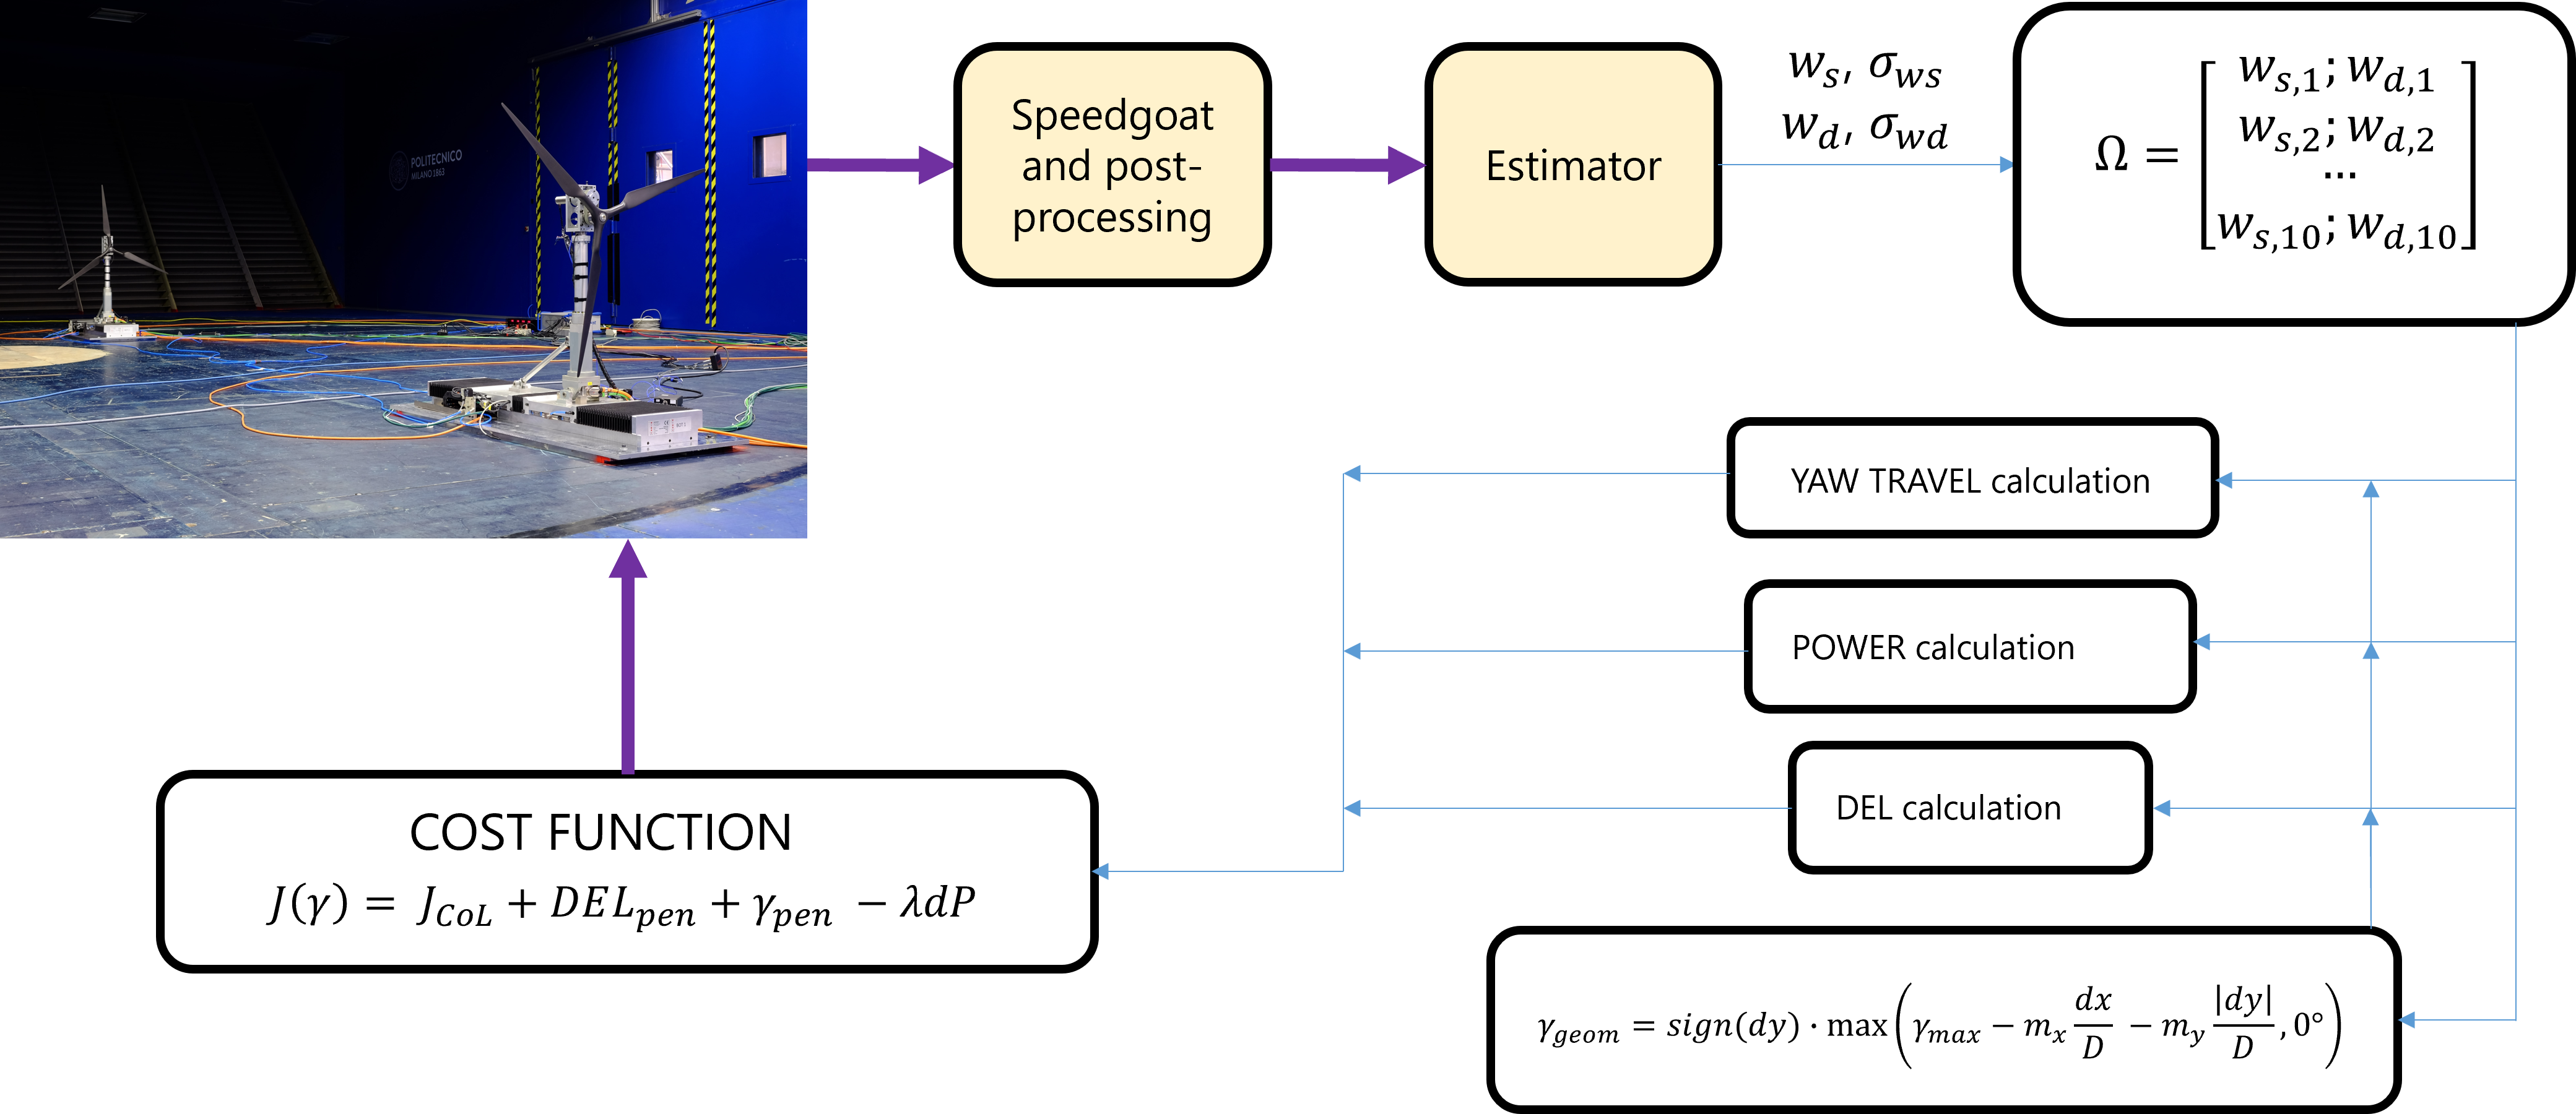
\includegraphics[width=\columnwidth]{pictures/optimization_scheme.png}
\caption{The architecture and workflow for the yaw selection.}
\label{fig:optimization_scheme}
\end{figure}



\subsection{FLORIDyn CLC and ZeroMQ model connection}
\label{sec:CLC_FLORIDyn}

Two different CLC implementations were developed in this work. The first consists of an offline implementation entirely within the FLORIDyn framework. In this approach, a FAST.Farm simulation is first performed and the resulting thrust time series are stored. During the offline phase, FLORIDyn receives the thrust values corresponding to each simulation time step and uses the EnKF to estimate the incoming wind speed, wind direction, and their associated uncertainties. Based on these estimates, the performance metrics presented in Section~\ref{sec:yaw_optimization} are evaluated and the cost function determines the optimal control action according to the selected optimization objective.

This offline implementation provides a convenient environment for controller development and tuning. Owing to the low computational cost of FLORIDyn, multiple simulations can be executed rapidly, enabling sensitivity analyses on the weighting coefficients of the cost function. This allows the controller to be tuned for different operational objectives, such as maximizing power production during periods of high electricity prices or reducing structural fatigue to extend the turbine lifetime when energy prices are lower.

The second implementation represents the online configuration and more closely reproduces the operation of a real wind farm. In this case, FLORIDyn is connected to FAST.Farm through the ZeroMQ communication interface available in FAST.Farm~\cite{rosco_docs_zeromq}, allowing yaw commands to be exchanged during the simulation. At each control time step, FAST.Farm transmits the required measurements (turbine thrust, generator power and wind direction) to FLORIDyn, which performs the estimation and optimization cycle illustrated in Figure~\ref{fig:optimization_scheme}. The optimal yaw command obtained by minimizing the cost function is then transmitted back to FAST.Farm and immediately applied to the running simulation.

In practice, the online configuration is deployed as a set of independent, concurrently running FLORIDyn--FAST.Farm co-simulation instances, each identified by a dedicated ZeroMQ port/case ID in the 15001--15011 range (ten cases in total, as one identifier in that range is reserved and unused). Each instance pairs one FAST.Farm simulation with its own FLORIDyn controller process, so that a full case study---covering different cost-function weightings and/or turbine layouts---can be executed in parallel rather than sequentially. This is the configuration used to obtain the case study of Section~\ref{sec:results}, where the five $\boldsymbol{\lambda}$ configurations of Table~\ref{tab:lambda_configurations} are each run as a separate, independently addressable ZeroMQ instance.

This online implementation reproduces the typical workflow of a real wind farm controller, where field measurements are continuously acquired, processed, and used to compute updated control actions. Consequently, it provides a realistic platform for assessing the proposed control strategy under real-time constraints and constitutes the basis for future experimental validation in scaled wind farm tests.



%% ===========================================================
%% ===========================================================

%  Results

\section{Results}
\label{sec:results}

\subsection{Floater implementation in FLORIDyn and effect on vertical deflection}

The implementation of the floater produces a pitch tilt on the platform, resulting in a tilted rotor and a vertical deflection of the wake centerline. This behaviour is shown in Figure~\ref{fig:vert_def}, where the wake centerline is deflected upward.


\begin{figure}[t]
\centering
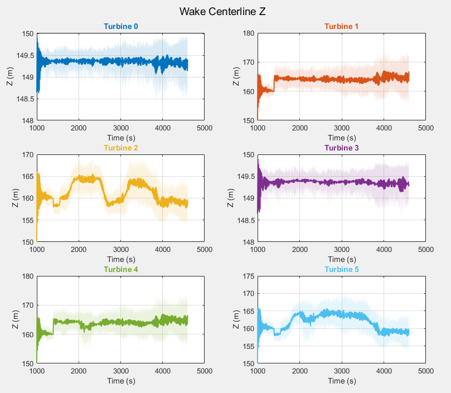
\includegraphics[width=\columnwidth]{pictures/vert_def.png}
\caption{Center of the wake at each turbine location: vertical wake deflection represantation.}
\label{fig:vert_def}
\end{figure}



\subsection{Case study}

To compare the effect of the cost-function weights on wake-steering behavior, five different simulations were run. In these simulations, the weights varied are those on the tower and blade load components and on the power production term; the tested combinations are reported in Table~\ref{tab:lambda_configurations}. The sea state was chosen with a significant wave height of 3\,m and a peak period of 8\,s, with wave direction aligned with the wind direction. The wind speed is 8\,$\mathrm{m/s}$.

\begin{table}[h]
\centering
\caption{Tested $\lambda$ configurations in the cost function.}
\label{tab:lambda_configurations}
\begin{tabular}{l | c c c}
\hline
\textbf{Run} & $\boldsymbol{\lambda^{\mathrm{twr}}}$ & $\boldsymbol{\lambda^{\mathrm{bld}}}$ & $\boldsymbol{\lambda^{\mathrm{pow}}}$ \\
\hline
1 & 0 & 0 & 1 \\
2 & 1 & 0 & 1 \\
3 & 1 & 1 & 1 \\
4 & 1 & 1 & 0 \\
5 & 1 & 1 & 5 \\
\hline
\end{tabular}
\end{table}

This set of configurations was applied to two mirrored turbine layouts, in order to assess how the resulting DEL magnitude depends on the layout.

In addition, a sixth, baseline configuration with no active yaw control was simulated, to serve as a reference for the power values obtained with wake steering.

Since DEL can also be computed directly from the FAST.Farm simulation, the actual DEL values were investigated as well and compared against those obtained from the surrogate DEL model implemented in FLORIDyn. The results show a different behavior depending on the yaw direction of the turbines. This asymmetry is also observed in the FAST.Farm DEL calculation, indicating that the load surrogate model correctly captures this non-symmetric behavior in the tower and blade DEL.


\subsection{Power and DEL resulting from the simulation}

The selected yaw values and the resulting power for each run are presented in the histograms of Figures~\ref{fig:histogram_power} and~\ref{fig:histogram_yaws}, which clearly show how the penalty weights affect the choice of yaw angle, which in turn directly affects power production. When $\lambda^{\mathrm{twr}}$ and/or $\lambda^{\mathrm{bld}}$ is set to 1, the yaw offsets are reduced and the power gain is minimal. When both load weights are 0 and $\lambda^{\mathrm{pow}}=1$ (Run 1), the power gain is maximum.

Another interesting case occurs when $\lambda^{\mathrm{pow}}=0$ and $\lambda^{\mathrm{twr}}=\lambda^{\mathrm{bld}}=1$ (Run 4): here we observe the minimum yaw offset and the smallest power increment.

Regarding the loads, a comparison of the DEL values computed in FLORIDyn is presented in Figure~\ref{fig:loads_FLORIDyn}, where the loads increase with increasing yaw offset. Furthermore, DEL was also computed directly from FAST.Farm and compared against the surrogate-model estimates from FLORIDyn.

\subsection{yaw effect on the structure}
Inserire postprocess di FASTfarm dove si comparano i moti della struttura nell varie simulazioni.

\section{Conclusions}

This work presents a digital twin framework for the real-time control of floating offshore wind farms, designed to operate under time-varying and uncertain environmental conditions. The proposed system integrates a dynamic low-fidelity wake model (FLORIDyn), extended to account for floating platform dynamics and vertical wake deflection, with a DEL surrogate model for fast structural load evaluation.

The framework operates using a thrust-based formulation, improving physical consistency for floating and scaled experimental setups. Wind direction uncertainty is explicitly handled through an Ensemble Kalman Filter, which provides probabilistic wind condition estimates used to compute risk-aware yaw setpoints via the $J_CoL_DEL$ cost function. The geometric yaw approach enables rapid candidate evaluation, meeting the real-time constraints imposed by wind tunnel scaling (0.25 s per iteration).

The modeling choices adopted in this work were made considering the possibility of transferring the framework from a simulated environment to the real wind farm setup at the GVPM facility of Politecnico di Milano. In light of this choice, it is important to mention that the geometric yaw selection is not an optimization algorithm, but rather, as suggested by the name, an instantaneous yaw selector based on the geometry of the wind farm. This choice was motivated by the compressed time scale imposed by the wind tunnel environment. In real wind farm operations, the considered time horizon would allow a computational time of approximately 15 s, enabling the use of actual optimization algorithms such as the widely adopted Serial Refine method, which could provide better-optimized setpoints for the wind farm.

As expected, the results show that wake steering control leads to an increase in structural loads, highlighting the need for load-aware optimization strategies and confirming that the load surrogate model can correctly replicate the physical phenomenon of load increase during wake steering operation.

Future work will focus on the experimental validation of the closed-loop controller in a wind tunnel environment. Additionally, the control framework will be extended to include induction control for fully aligned turbine configurations, with the aim of reducing structural loads under full-wake conditions. Further effort will also be directed toward demonstrating that continuously optimizing wind farm operation can provide measurable benefits over longer time horizons.


\appendix
\section{Example Appendix Section}
\label{app1}

Appendix text.

\bibliographystyle{elsarticle-num} 
\bibliography{Digital_twin_references}

\end{document}
